\documentclass[a4paper,14pt]{extreport}
\usepackage[left=1.5cm,right=1.5cm,
    top=1.5cm,bottom=2cm,bindingoffset=0cm]{geometry}
\usepackage{scrextend}
\usepackage[T1,T2A]{fontenc}
\usepackage[utf8]{inputenc}
\usepackage[english,russian,ukrainian]{babel}
\usepackage{tabularx}
\usepackage{amssymb}
\usepackage{color}
\usepackage{amsmath}
\usepackage{mathrsfs}
\usepackage{listings}
\usepackage{graphicx}
\graphicspath{ {./images/} }
\usepackage{lipsum}
\usepackage{xcolor}
\usepackage{hyperref}
\usepackage{tcolorbox}
\usepackage{tikz}
\usepackage[framemethod=TikZ]{mdframed}
\usepackage{wrapfig,boxedminipage,lipsum}
\mdfdefinestyle{MyFrame}{%
linecolor=blue,outerlinewidth=2pt,roundcorner=20pt,innertopmargin=\baselineskip,innerbottommargin=\baselineskip,innerrightmargin=20pt,innerleftmargin=20pt,backgroundcolor=gray!50!white}
 \usepackage{csvsimple}
 \usepackage{supertabular}
\usepackage{pdflscape}
\usepackage{fancyvrb}
%\usepackage{comment}
\usepackage{array,tabularx}
\usepackage{colortbl}
\usepackage{fp}

\usepackage{varwidth}
\tcbuselibrary{skins}
\usepackage{fancybox}


\usepackage{tikz}
\usepackage[framemethod=TikZ]{mdframed}
\usepackage{xcolor}
\usetikzlibrary{calc}
\makeatletter
\newlength{\mylength}
\xdef\CircleFactor{1.1}
\setlength\mylength{\dimexpr\f@size pt}
\newsavebox{\mybox}
\newcommand*\circled[2][draw=blue]{\savebox\mybox{\vbox{\vphantom{WL1/}#1}}\setlength\mylength{\dimexpr\CircleFactor\dimexpr\ht\mybox+\dp\mybox\relax\relax}\tikzset{mystyle/.style={circle,#1,minimum height={\mylength}}}
\tikz[baseline=(char.base)]
\node[mystyle] (char) {#2};}
\makeatother

\definecolor{ggreen}{rgb}{0.4,1,0}
\definecolor{rred}{rgb}{1,0.1,0.1}
\definecolor{amber}{rgb}{1.0, 0.75, 0.0}
\definecolor{babyblue}{rgb}{0.54, 0.81, 0.94}
\definecolor{amethyst}{rgb}{0.6, 0.4, 0.8}

\usepackage{float}
\usepackage{wrapfig}
\usepackage{framed}
%for nice Code{
\lstdefinestyle{customc}{
  belowcaptionskip=1\baselineskip,
  breaklines=true,
  frame=L,
  xleftmargin=\parindent,
  language=C,
  showstringspaces=false,
  basicstyle=\small\ttfamily,
  keywordstyle=\bfseries\color{green!40!black},
  commentstyle=\itshape\color{purple!40!black},
  identifierstyle=\color{blue},
  stringstyle=\color{orange},
}
\lstset{escapechar=@,style=customc}
%}


\begin{document}
\pagecolor{white}

%----------------------------------------1
\newtcbox{\xmybox}[1][red]{on line, arc=7pt,colback=#1!10!white,colframe=#1!50!black, before upper={\rule[-3pt]{0pt}{10pt}},boxrule=1pt, boxsep=0pt,left=6pt,right=6pt,top=2pt,bottom=2pt}



\begin{titlepage}
  \begin{center}
    \large
    Національний технічний університет України \\ "Київський політехнічний інститут імені Ігоря Сікорського"


    Факультет Електроніки

    Кафедра мікроелектроніки
    \vfill

    \textsc{ЗВІТ}\\

    {\Large Про виконання лабораторної роботи №6\\
      з дисципліни: «Твердотільна електроніки-1»\\[1cm]

      «ІНТЕГРАЛЬНІ СХЕМИ СТАТИЧНОЇ ЛОГІКИ НА МДН – ТРАНЗИСТОРАХ» \\

    }
  \bigskip
\end{center}
\vfill

\newlength{\ML}
\settowidth{\ML}{«\underline{\hspace{0.4cm}}» \underline{\hspace{2cm}}}
\hfill
\begin{minipage}{1\textwidth}
Виконавець:\\
Студент 3-го курсу \hspace{4cm} $\underset{\text{(підпис)}}{\underline{\hspace{0.2\textwidth}}}$  \hspace{1cm}А.\,С.~Мнацаканов\\
\vspace{1cm}

Превірив: \hspace{6.1cm} $\underset{\text{(підпис)}}{\underline{\hspace{0.2\textwidth}}}$  \hspace{1cm}Л.\,М.~Королевич\\

\end{minipage}

\vfill

\begin{center}
2021
\end{center}
\end{titlepage}
%---------------------------------------------------------------------------------------------------------------------------------------------------------------------------------



\begin{center}1. МЕТА РОБОТИ\\ \end{center}

Вивчення будови, методів виготовлення, основних характеристик і технічних параметрів інтегральних МДН-транзисторів.

\begin{center}2. ЗАВДАННЯ\\ \end{center}


1.Виконати вимірювання сімейства характеристик передачі - залежності струму стоку від напруги затвор-виток інтегрального МДН-транзистора: $\mathrm{Ic}($ Езв $),$ при Еc=const. Побудувати характеристики передачі на одному малюнку.\\

2.Виконати вимірювання вихідних характеристик - залежності струму стоку від напруги сток-виток: $-\mathrm{Ic}(\mathrm{EcB}),$ при Ез= const Побудувати сімейство вихідних характеристик.\\

3.Побудувати графік залежності $\sqrt{I_{C}\left(E_{3 B}\right)}$ у пологій області вихідних характеристик та графічно визначити порогову напругу МДН-транзистора.\\

4.Визначити крутизну, динамічний опір стоку, коефіцієнт підсилення напруги для крутої для пологої областей вихідних характеристик транзистора $\left(\mathrm{S} 1 ; \mathrm{S} 2, \mathrm{rc} 1 ; \mathrm{rc} 2 ; \mu_{1} ; \mu_{2}\right)$\\

5.3апропонуйте заходи щодо підвищення частоти Г$_{\text{верх}}$, зниження порогової напруги та зменшення паразитних ємностей інтегрального МДН-транзистора.\\

\newpage
\begin{center}2.1. Установка і Таблиці\\ \end{center}
%---------------------------------------------------------------------------------------------------------------------------------------------------------------------------------
\begin{figure}[h]
\center{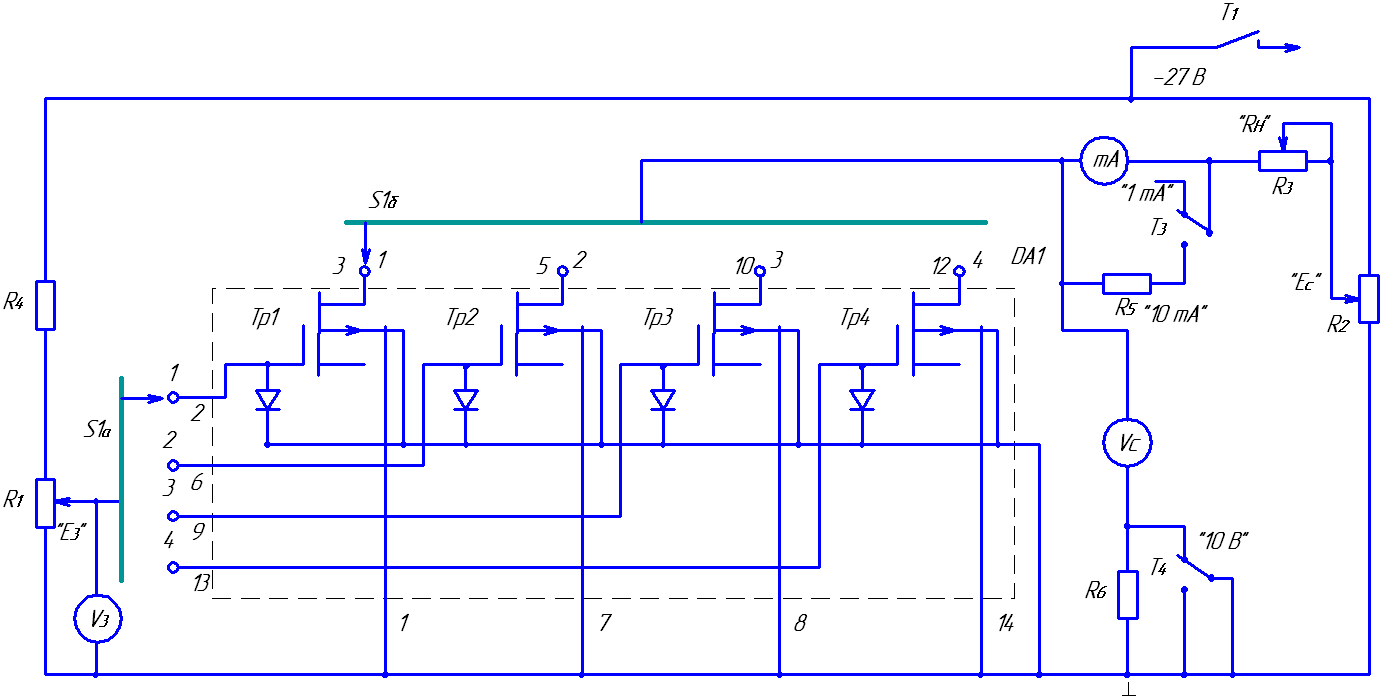
\includegraphics[width=0.8\linewidth]{s.png}}
\caption{ДОСЛІДНА УСТАНОВКА К168КТ2А.}
\label{ris1}
\end{figure}

\newpage



\begin{landscape}
  \begin{center}Табл. 1: Значення для сімейства характеристик передачі.\end{center}
  \begin{figure}[h]
    \center{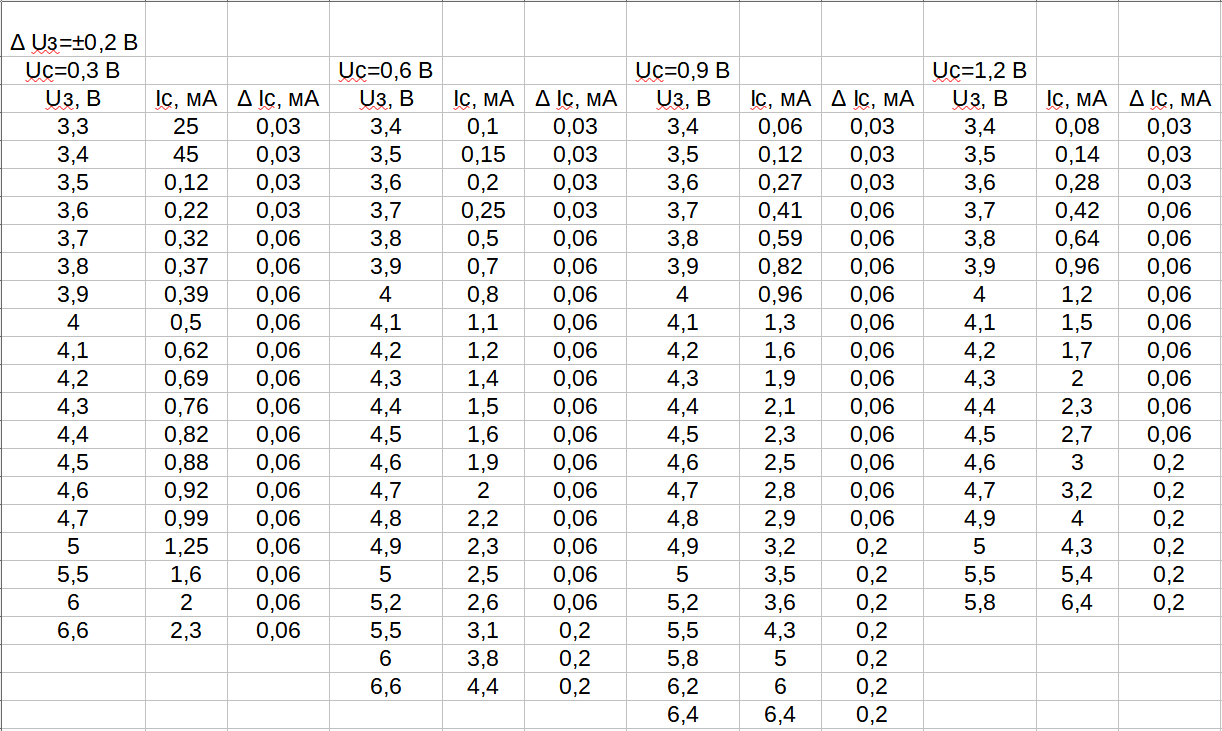
\includegraphics[width=0.8\linewidth]{t1.png}}

  \end{figure}
\newpage
  \begin{center}Табл. 2:Вихідні характеристики, залежності струму стоку від напруги сток-виток.\end{center}
  \begin{figure}[h]
    \center{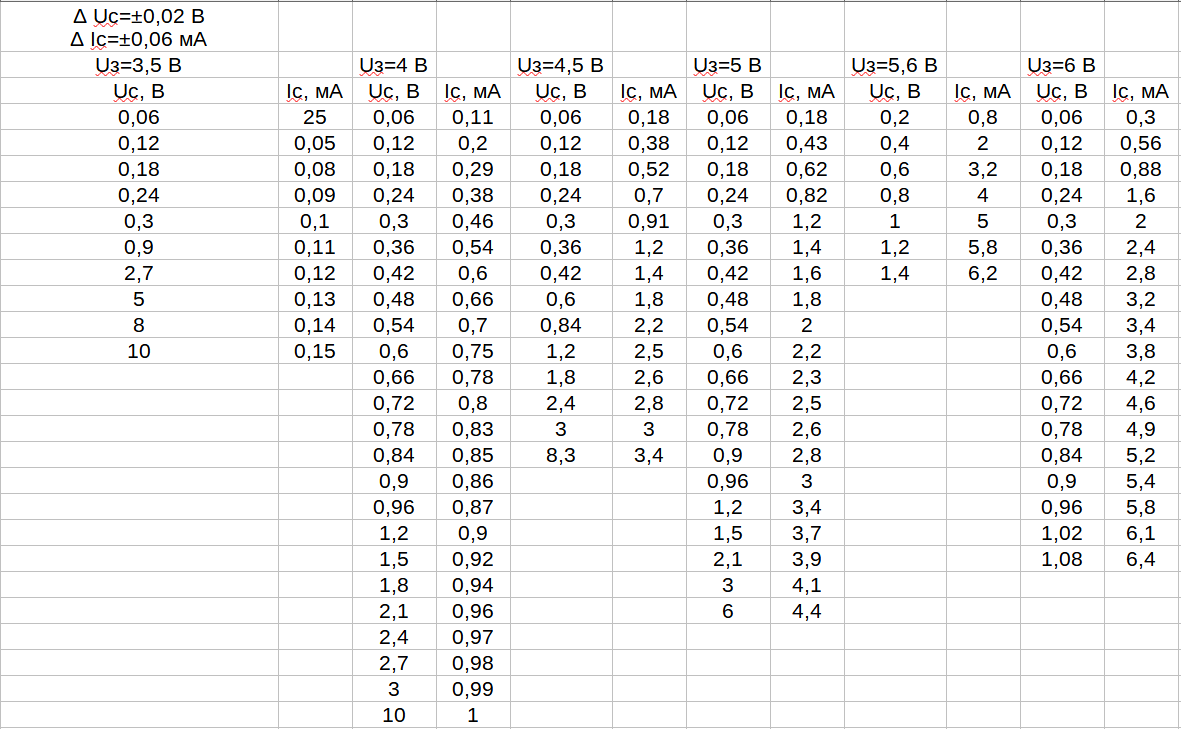
\includegraphics[width=0.8\linewidth]{t2.png}}
  \end{figure}
\end{landscape}


\newpage
\clearpage

\begin{center}3.  Графіки\\ \end{center}
\begin{figure}[h]
\center{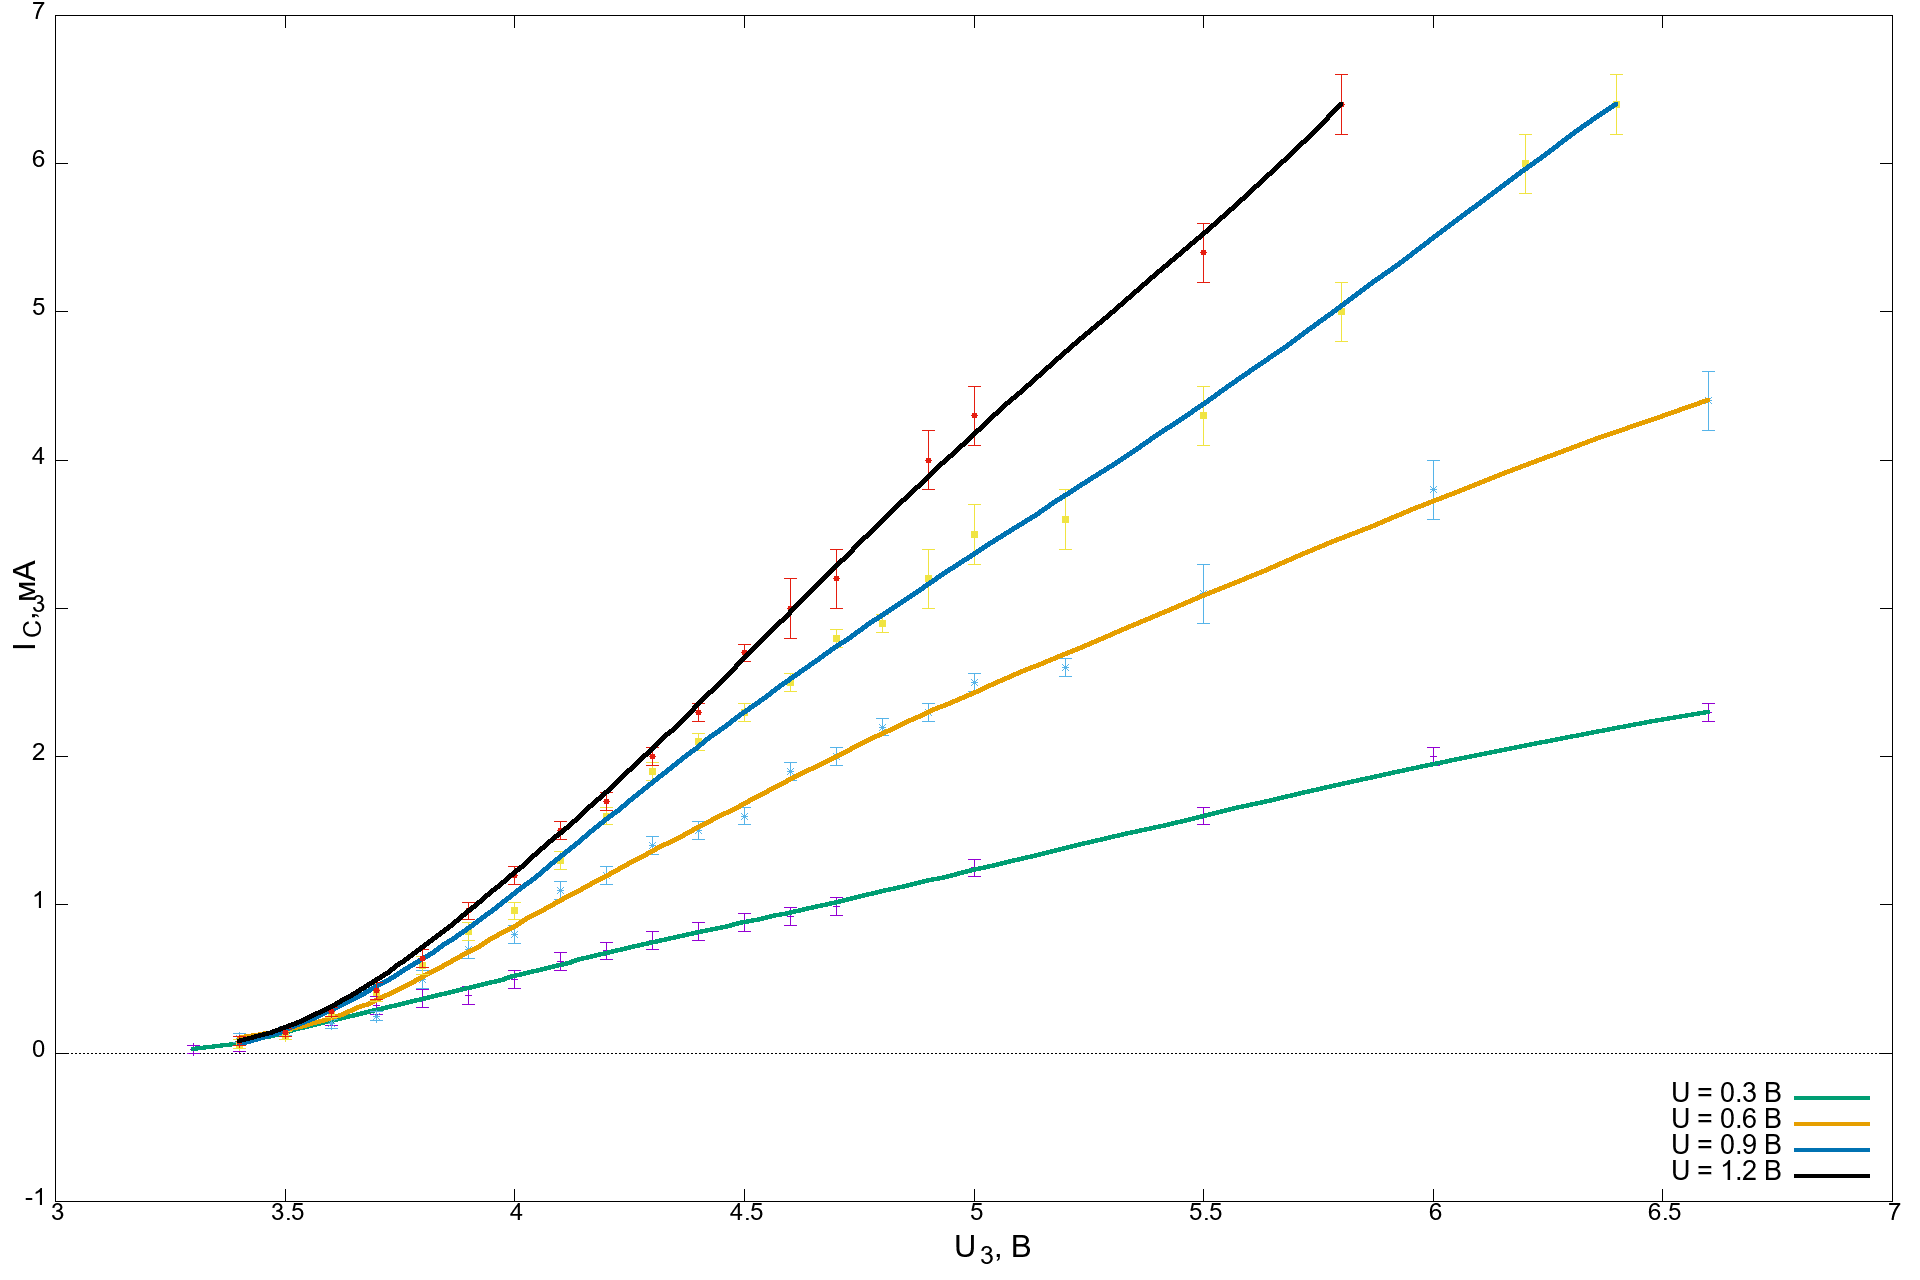
\includegraphics[width=0.7\linewidth]{1.png}}
\caption{Сімейство характеристик передачі.}
\label{ris2}
\end{figure}

\begin{figure}[h]
\center{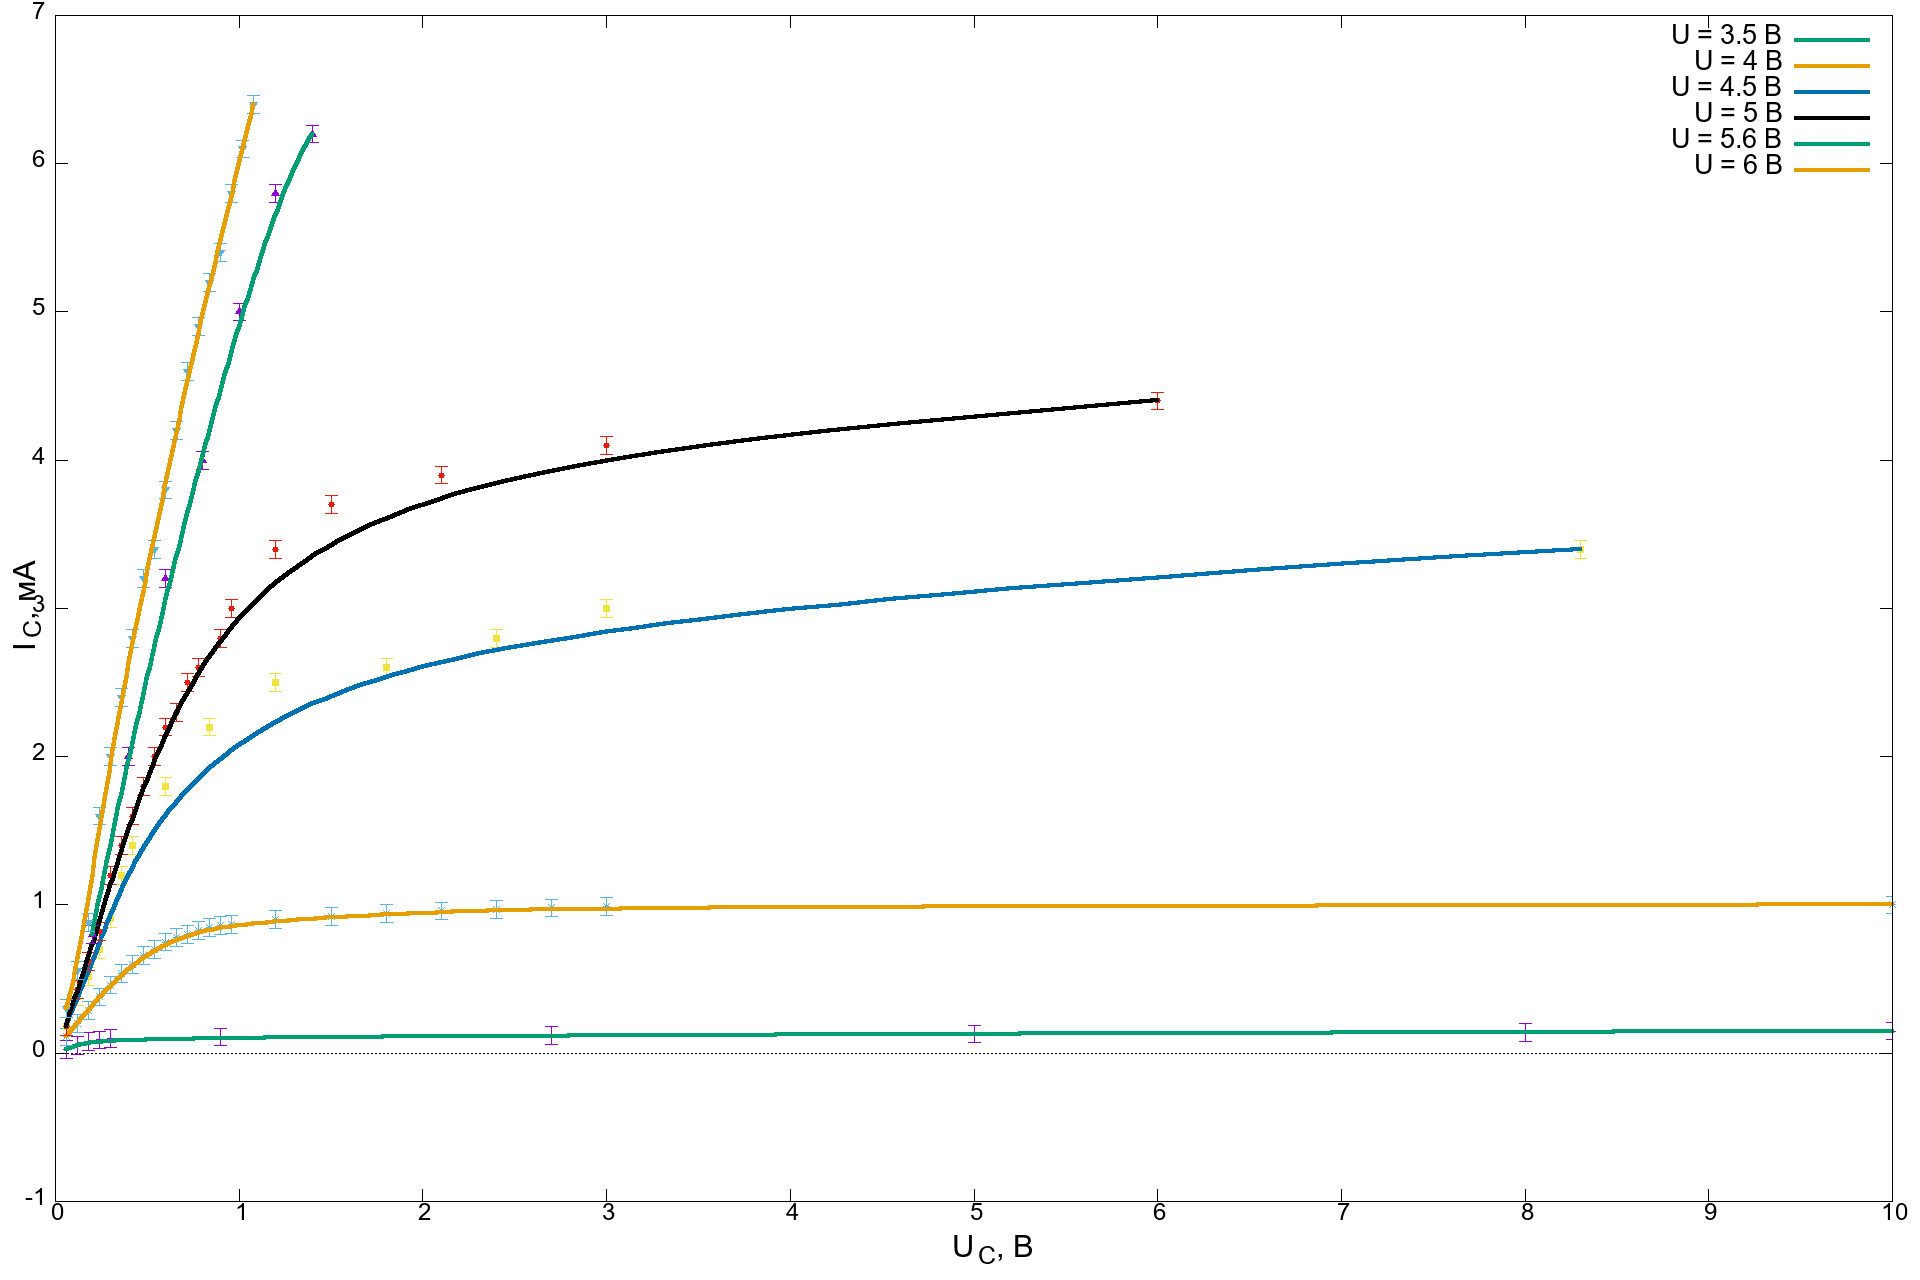
\includegraphics[width=0.7\linewidth]{2.png}}
\caption{Сімейство вихідних характеристик транзистора.}
\label{ris3}
\end{figure}

\begin{figure}[h]
\center{
\includegraphics[width=0.8\linewidth]{3.pdf}}
\caption{.Графік для визначення порогової напруги.}
\label{ris5}
\end{figure}

\begin{figure}[h]
\center{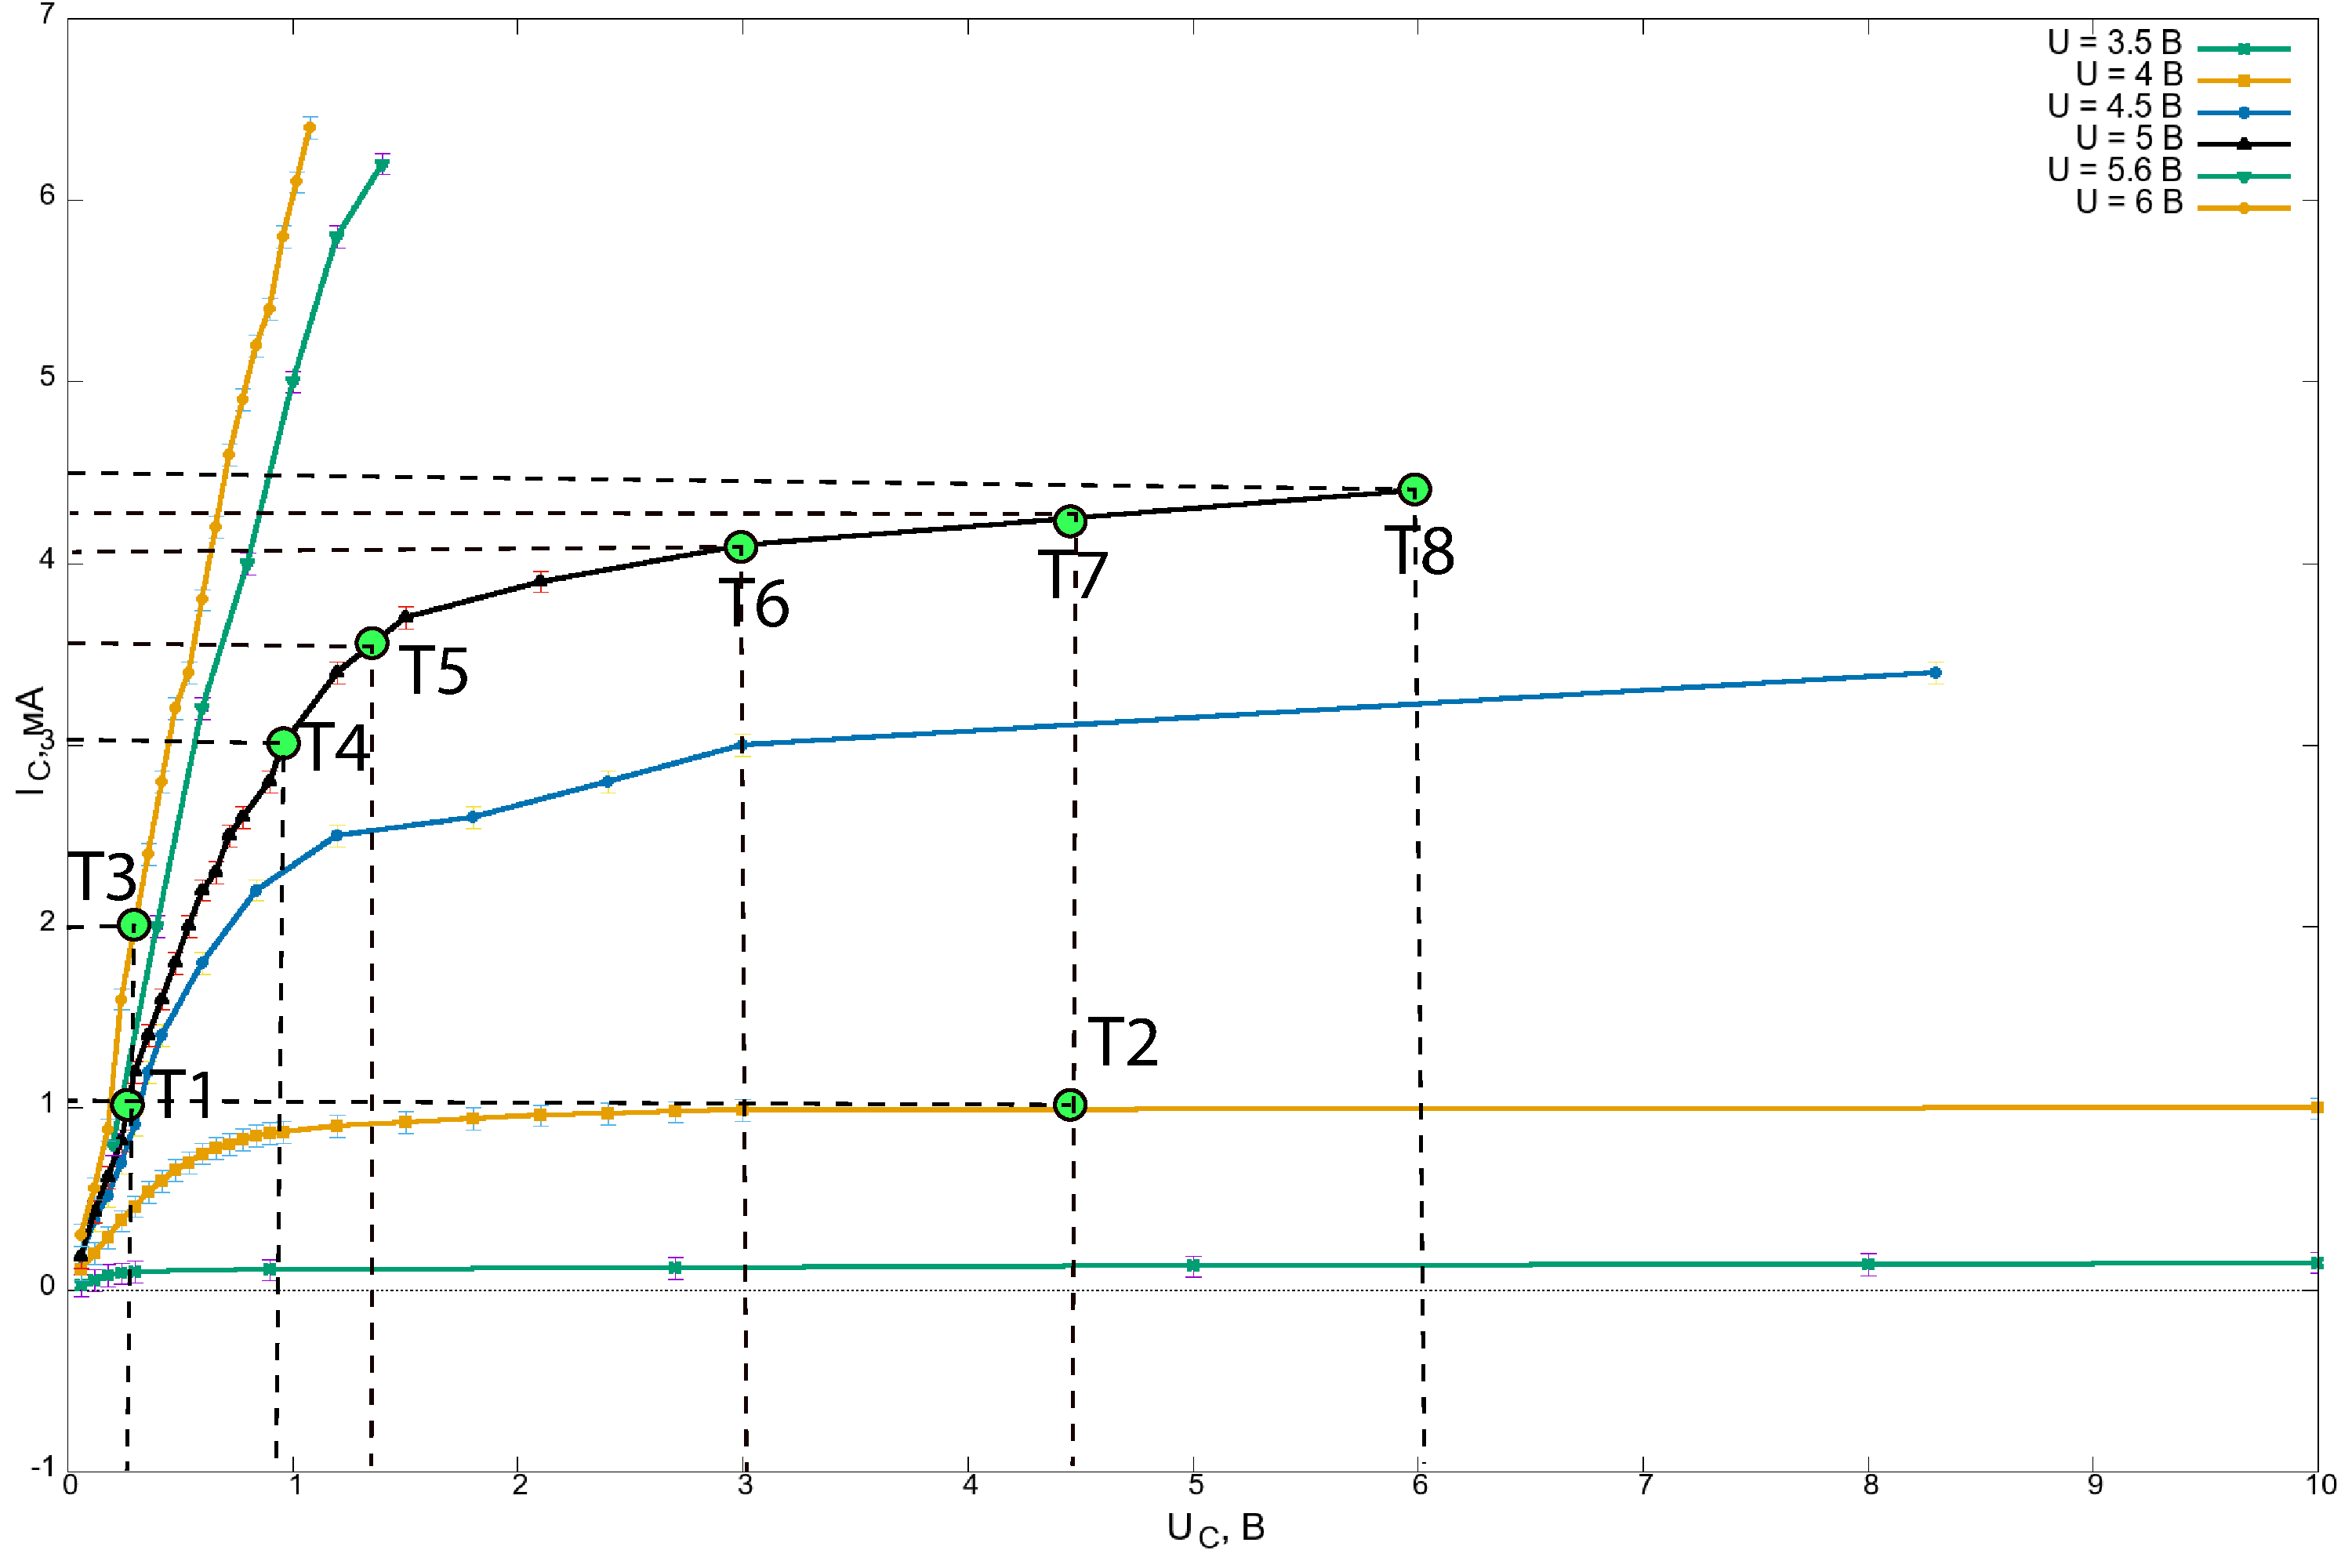
\includegraphics[width=0.8\linewidth]{2.pdf}}
\caption{Графік з точками для розрахунку параметрів}
\label{ris6}
\end{figure}


\newpage
\clearpage

\begin{center}4. Розрахунки\\ \end{center}

Взявши корінь з $I_C$  та побудувавши график (рис.\ref{ris5}) можу визначити порогову напругу, яка = 3,2 В.\\
За допомогою точок Т1 та Т2 на рис.\ref{ris6} крутизну характеристики, використовуючи наступну формулу:
\begin{align}\label{q1}
  S = \dfrac{\triangle I_C}{\triangle U_{\text{3}}} = 0,81 \dfrac{\text{мА}}{\text{В}}
\end{align}
За допомогою точок Т5 та Т4 знайду внутрішній диференційний опір:
\begin{align}\label{q2}
  r_i = \dfrac{\triangle U_{BC}}{\triangle I_{C_2}} = 1000 \text{Ом}
\end{align}
За допомогою S та $r_i$ знайду граничний кофіцієнт підсилення за напругою:
\begin{align}\label{q3}
  \mu_1 = S\cdot r_i = 0,81
\end{align}

\begin{center} ТЕПЕР ДЛЯ ПОЛОГОЇ ОБЛАСТІ \end{center}

\begin{align}\label{q4}
  S = \dfrac{\triangle I_C}{\triangle U_{\text{3}}} = 3 \dfrac{\text{мА}}{\text{В}}
\end{align}
За допомогою точок Т5 та Т4 знайду внутрішній диференційний опір:
\begin{align}\label{q5}
  r_i = \dfrac{\triangle U_{BC}}{\triangle I_{C_2}} = 6000 \text{Ом}
\end{align}
За допомогою S та $r_i$ знайду граничний кофіцієнт підсилення за напругою:
\begin{align}\label{q6}
  \mu_1 = S\cdot r_i = 18
\end{align}





















\begin{center}5. Висновок\\ \end{center}

У даній лабораторній роботі було виміряно характеристики передачі та
вхідні характеристики МДН-транзистора. За отриманими
даними з графіку я (як показанов прикладі) визначив порогову напруга Uпор, потім за формулами розрахував крутизну
S, динамічний опір $r_i$ та коефіцієнт підсилення напруги для
лінійної та пологої ділянок ВАХ. На мою думку для зниження порогової напруги потрібно як підзасліний шар
використовувати $Si_3N_4$ (нітрид кремнію), а для зменшення паразитних ємностей до металічних елементів можна додати
ще один заземлений екран та скоби з нікелевого сплаву.


\end{document}
